%\documentclass[12pt,preprint]{aastex}
\documentclass{emulateapj}
%\usepackage{apjfonts}
\usepackage{amsmath}
\usepackage{natbib}
\usepackage{graphicx}
\usepackage{bm}

\slugcomment{}

%% macros
\newcommand\da{\delta\!\alpha}
\newcommand\ks{\kappa_s}
\newcommand\ps{\phi_{\rm sub}}
\newcommand\mathbi[1]{\textbf{\em #1}}
\newcommand\rv{\bm r}
\newcommand\xv{\bm x}
\newcommand\uv{\bm u}
\newcommand\du{\delta\uv}
\newcommand\av{\bm \alpha}
\newcommand\dphi{\delta\phi}
\newcommand\dtau{\delta\tau}
\newcommand\avg[1]{\left\langle{#1}\right\rangle}
\newcommand\Rein{R_{\rm Ein}}
\newcommand\Sigcr{\Sigma_{\rm crit}}
\newcommand\tot{{\rm tot}}
\newcommand\mhat{{\hat m}}

\shorttitle{Inferring Time Delays in Strong Lenses}
\shortauthors{Leonidas A.~Moustakas \& Andrew~Romero-Wolf}

\begin{document}

\title{Bayesian Inference Time Delay Recovery for Strong Gravitational Lenses}

\author{Leonidas A. Moustakas \& Andrew Romero-Wolf\altaffilmark{1}}
\altaffiltext{1}{Jet Propulsion Laboratory, California Institute of
  Technology, 4800 Oak Grove Dr, MS 169-506, Pasadena, CA 91109} 

\begin{abstract}
  Gravitational  lensing  on   astronomical  scales.  Methodology  for
  inferring time delays in time-streams of photometric measurements in
  a multiply  imaged quasar.  Bayesian inference.  Comparison to other
  techniques  including matrix  inversion.  Realistic  simulated light
  curves  produced, and  recovery efficiency  systematically explored,
  marginalizing over  the nuisance  parameters of the  parameters that
  control the behavior of  the light curves.  Microlensing effects and
  considerations.  Main conclusions.
\end{abstract}
 
\keywords{gravitational lensing --- cosmology: dark matter} 

\section{Introduction}

% \begin{equation}
% {\rm S} = {{D_{\rm ang}(z_{\rm cluster}, z_{\rm target})}\over{D_{\rm ang}(z_{\rm target})}} 
%               {{D_{\rm ang}(z_{\rm model})}\over{D_{\rm ang}(z_{\rm cluster},z_{\rm model})}}. 
% \end{equation}

% \begin{figure*}[t]
% \begin{center}
% \plotone {figures/magfig_macs1149_11495_z9p7LAST.png}
% \caption{MACS 1149. Top left: The \emph{HST} ACS and WFC3 mosaic
%   footprint (inner and outer polygons), used to calculate the area
%   accessed by each. The image is the segmentation map. Remaining three
%   panels: The magnification map for source at the redshifts indicated,
%   with magnification strength shown in the bar on the right.
% }\label{fig:macs1149}
% \end{center}
% \end{figure*}

% \begin{figure}[t]
% \begin{center}
% \plotone{figures/mastervolume.png}
% %\includegraphics{../figures/b0712_model_for_masterlens.png}
% \caption{The cumulative volume accessible as a function of limiting
%   magnification, for a set of twelve CLASH clusters (and their sum). 
% }\label{fig:volume}
% \end{center}
% \end{figure}

Context. Lensing. Distances light travels, and differences in arrival
time versus relative distance differences.

History and realization. Power of time delays for H0, Refsdal, leading into modern
era of cosmology.  Relevance of lenses for present discussions of
cosmography, interesting tension between Planck and lensing results,
quote the results on that.  Potential improvement in quality of
results with greater time delay precision, in the limit of mass model
and environment characterization improvements. 

Looking into the future: Dark matter study, New Channel \citep{Keeton2009a}, driving us to
time delay precisions of hours or better.  Cf Oguri's compilation,
cosmograil precision from ground-based campaigns to date. Past and current work. 
Techniques generally developed to date, including interpolating, cross-correlations, maximum likelihood (Fasscnacht, COSMOGRAIL, Hojatti+Kim+Linder, others). Naturalness of setting up a Bayesian approach, if there is a clear predictive model for the time variations of quasar light curves. 

\subsection{Introducing RXJ1131}

Why it's an interesting target, H0, dark matter, observations with Hubble etc, models for it predicting its observational parameters including the time delays, the interesting thing pointed out in KM09 that an order-reversal could be quite interesting. 

Figures: HST and model plot. 

Possibly a table showing existing observations/measurements, drawn from literature. 

\subsection{Bayesian Analysis Framework}

Bayes rule, model and observational parameters, MCMC implementation. The things that we need -- ie a predictive model that connects the parameter sets, and an understanding of the obsrevational uncertainties.

\section{Simulating light curves}
\subsection{Quasar physics}

This is a key ingredient, since the physical structure of an accreting supermassive black hole determines the character of the light variations, and we need to get it right if we are forecasting how well we can recover information. 

Kelly's damped random walk technique, parametrization for the light curve generation and (brief) motivation/intperpretation of these parameters, literature vetting and testing these. 
\subsection{Observing cadences and campaigns}\label{}

Choices for observing campaigns (remember, this is just for straight light curves at the moment. )

Generally on how this may be set up for different circumstances, and what types of campaigns may apply to 1131, including what campaigns have been implemented (e.g. COSMOGRAIL). 

\subsection{Photometric uncertainties}\label{}

Random and systematic, possibility of covariances, and so on.  

Relative consequences or advantages of ground versus space. 

Table summarizing the cadence/campaign/uncertainty combinations we adopt in this paper. 

Figure of sample light curves and reconstructed parameters. 


\section{Measuring Time Delays}

The likelihood function used to reconstruct the quasar light curve damped random walk parameters is given by Kelly et al. 2009. Written as a log-likelihood
\begin{align} 
& \log\mathcal{L}_{K}(\langle m\rangle, \sigma,\tau | X) = \nonumber \\
& \ \ \ \ \ \ \ \ -\frac{1}{2}\sum_{i=1}^{n}\left\{
\frac{\left(\hat{x}_i-x^{*}_i\right)^2}{\Omega_i+\sigma_i^2} 
+ 
\log\left[2\pi\left(\Omega_i+\sigma_i^2\right)\right]
\right\}
\end{align}
where 
% \begin{equation}
\begin{alignat}{1}
& x_{i}^{*} = x_i-\langle m \rangle \\
& \hat{x}_0 = 0   \\
& \Omega_{0}=\frac{\tau\sigma^2}{2} \\
& \hat{x}_i = a_i\hat{x}_{i-1} + \frac{a_i\Omega_{i-1}}{\Omega_{i-1}+\sigma^2_{i-1}} \left(x^{*}_{i-1}-\hat{x}_{i-1}\right) \\
& \Omega_{i}=\Omega_{0}\left(1-a_{i}^2\right) + a_{i}^2\Omega_{i-1}\left(1-\frac{\Omega_{i-1}}{\Omega_{i-1}+\sigma_{i-1}^2}\right) \\
& a_i = e^{-\left(t_i-t_{i-1}\right)/\tau} \\
% & a_i = \exp\left(\frac{t_i-t_{i-1}}{\tau}\right) \\
\end{alignat}
The reconstruction of time-delays in this analysis relies on entirely on the physics of quasar light delay fluctuations. The light curves of two images of a quasar are merged according to hypothesized delay and magntide offset. A posterior probability is then calculated for the merged light curve under different hypotheses for the parameters $\langle m\rangle$, $\tau$, and $\sigma$.
\begin{align}
& \mathcal L (\Delta t, \Delta m, \sigma, \tau, \langle m \rangle | X_1, X_2)  = \nonumber \\
& \mathcal{L}_{K} \left( \sigma, \tau, \langle m \rangle  | M(\Delta t,\Delta m ; X_1, X_2) \right)
\end{align}

The posterior probability is given by
\begin{align}
& p(X_1, X_2 | \Delta t, \Delta m, \langle m \rangle, \sigma,\tau) \propto \nonumber \\
&  \ \ \ \ \ \ \mathcal{L}(\Delta t, \Delta m, \langle m \rangle, \sigma,\tau | X_1, X_2)\times p(\Delta t, \Delta m, \langle m \rangle, \sigma,\tau)
\end{align}
The assignement of priors is flat in $\Delta t$. The parameters $\sigma$ and $\tau$ are scale parameters so their priors are given by $p(\sigma)=\sigma^{-1}$ and $p(\tau)=\tau^{-1}$. The parameter $\langle m \rangle$ and $\Delta m$ are also scale parameters but they in logarithmic units and therefore are assigned flat priors.
\section{Running the Experiment}\label{}

Demonstrate how well we recover structural parameters we put in, showing triangle diagrams.


\begin{figure}[t]
\begin{center}
%\plotone{figures/mastervolume.png}
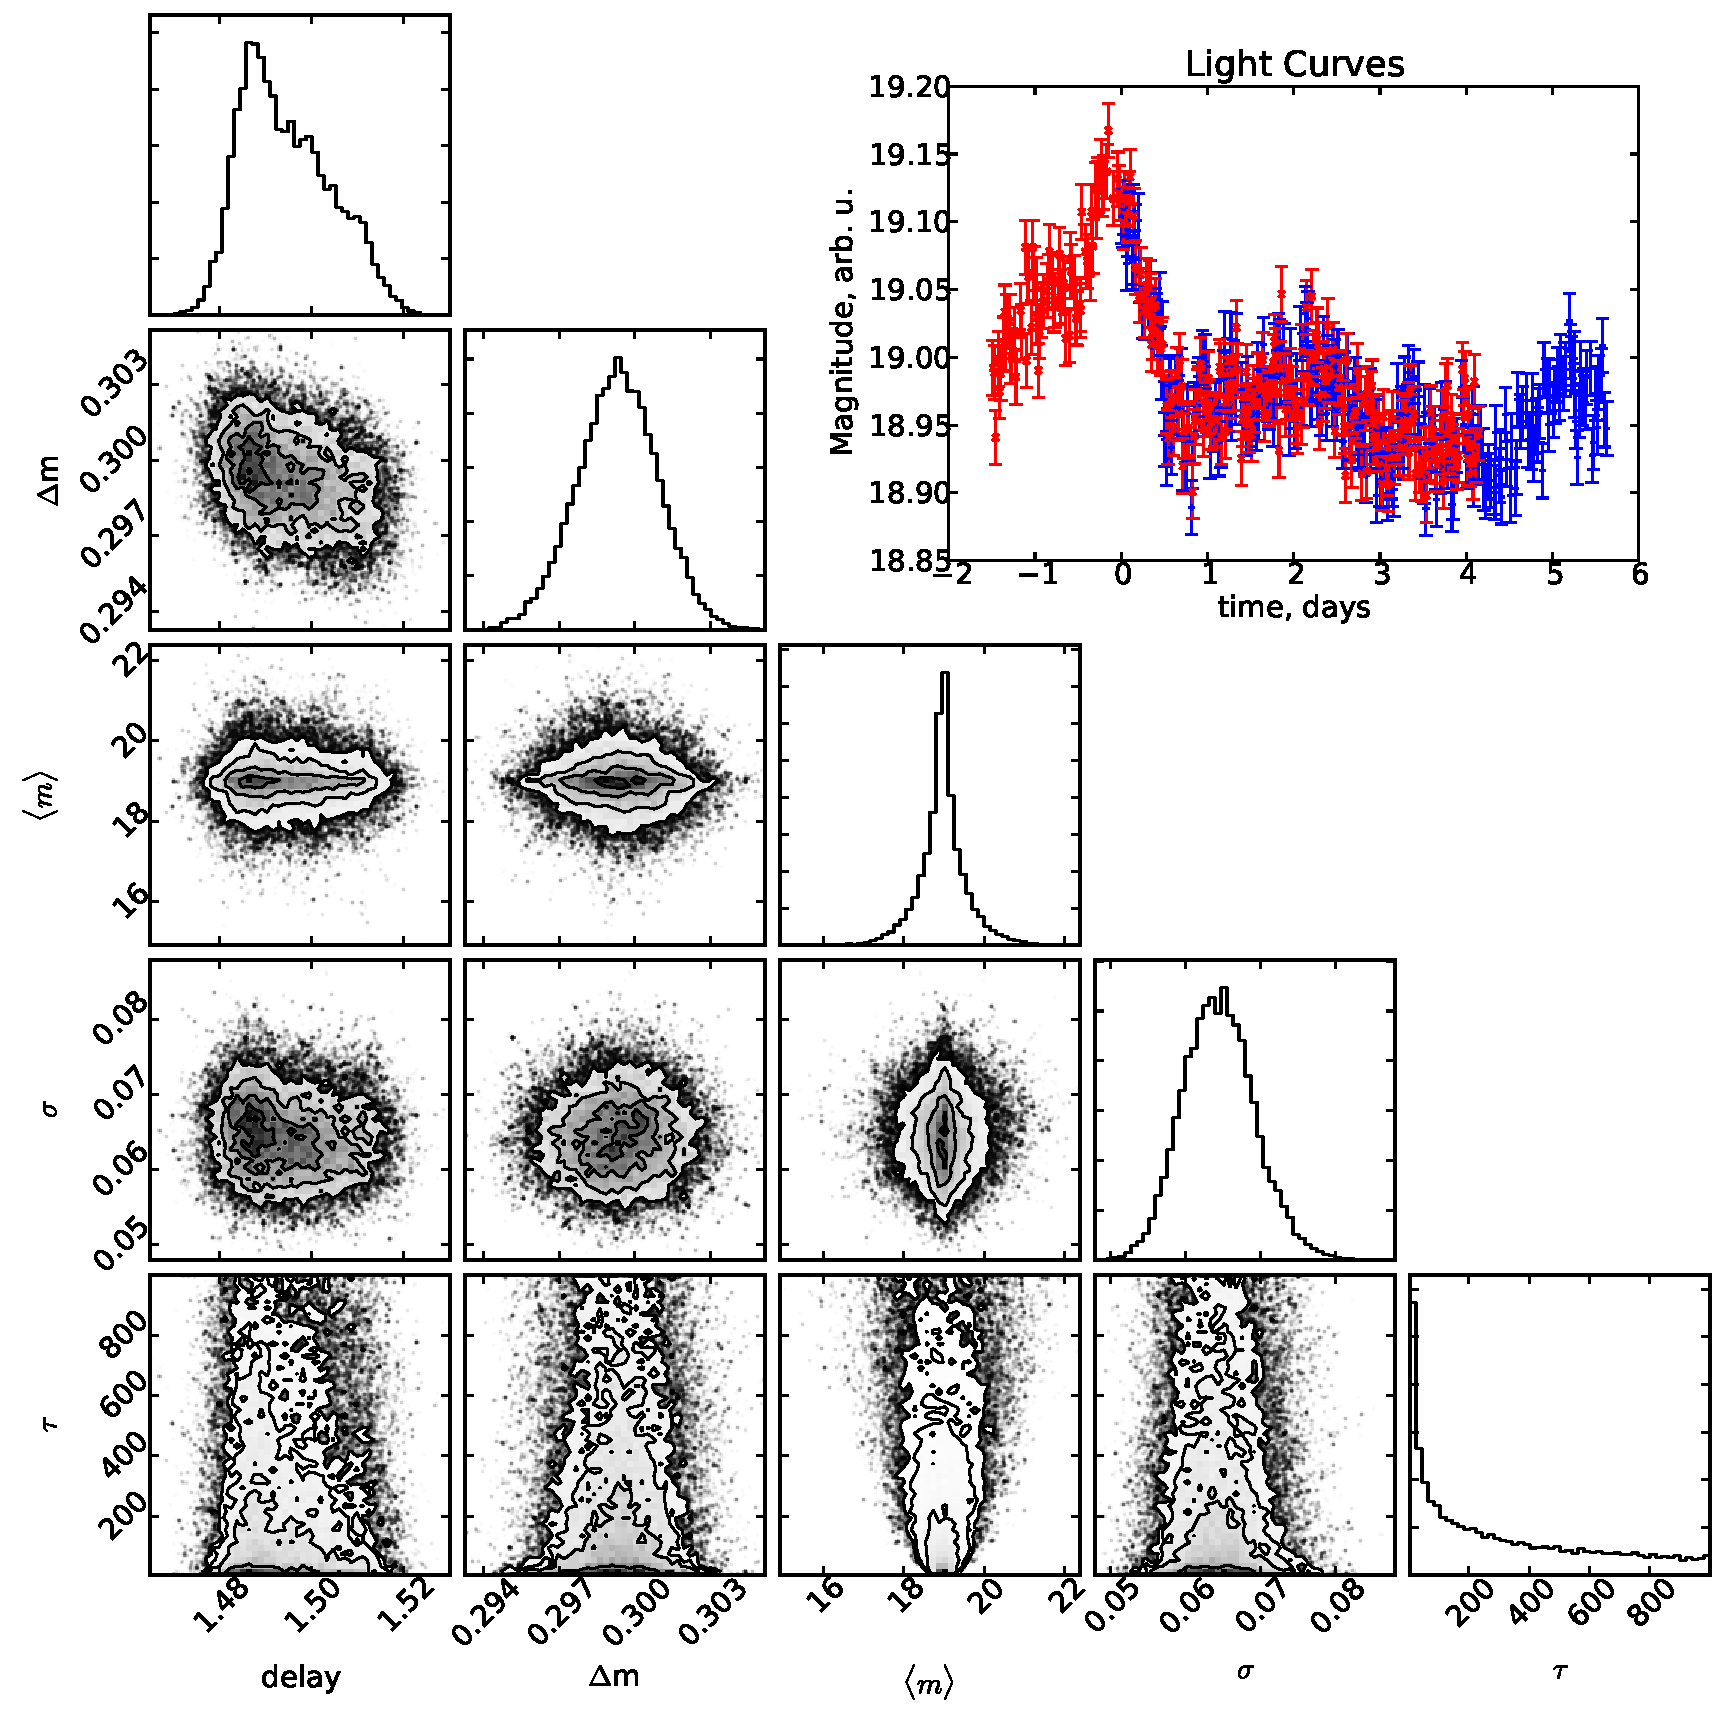
\includegraphics[width=\linewidth]{./triangle_example.pdf}
\caption{Markov chain Monte Carlo results for an example for the parameter reconstruction of a light curve and its delayed and magnitude offset image. The quasar light curve parameters $\tau$, $\sigma$ and $\rangle m \langle$ are estimated under a hypothesis value for the delay and $\Delta m$. On the top right the quasar light curve (blue) and its delayed magnitude offset image (red) are shown with the image delay and magnitude offset corrected from the most probable values of the delay and $\Delta m$ distributions.}\label{fig:volume}
\end{center}
\end{figure}


The cuts required by for a valid reconstruction are described as follows. We fit a Gaussian curve to the distribution of 100 simulation delay results. We have found that the python SciPy curve\_fit method, which employs the Levenberg-Marquardt algorithm, is not driven by outliers. The standard deviation $\sigma$ from the fit is used to reject reconstruction results by requiring that a reconstructed delay be within 3$\sigma$ of the true delay. We also require that the uncertainty in the delay be within 3$\sigma$ to reject poor reconstructions.



\begin{figure}[t]
\begin{center}
%\plotone{figures/mastervolume.png}
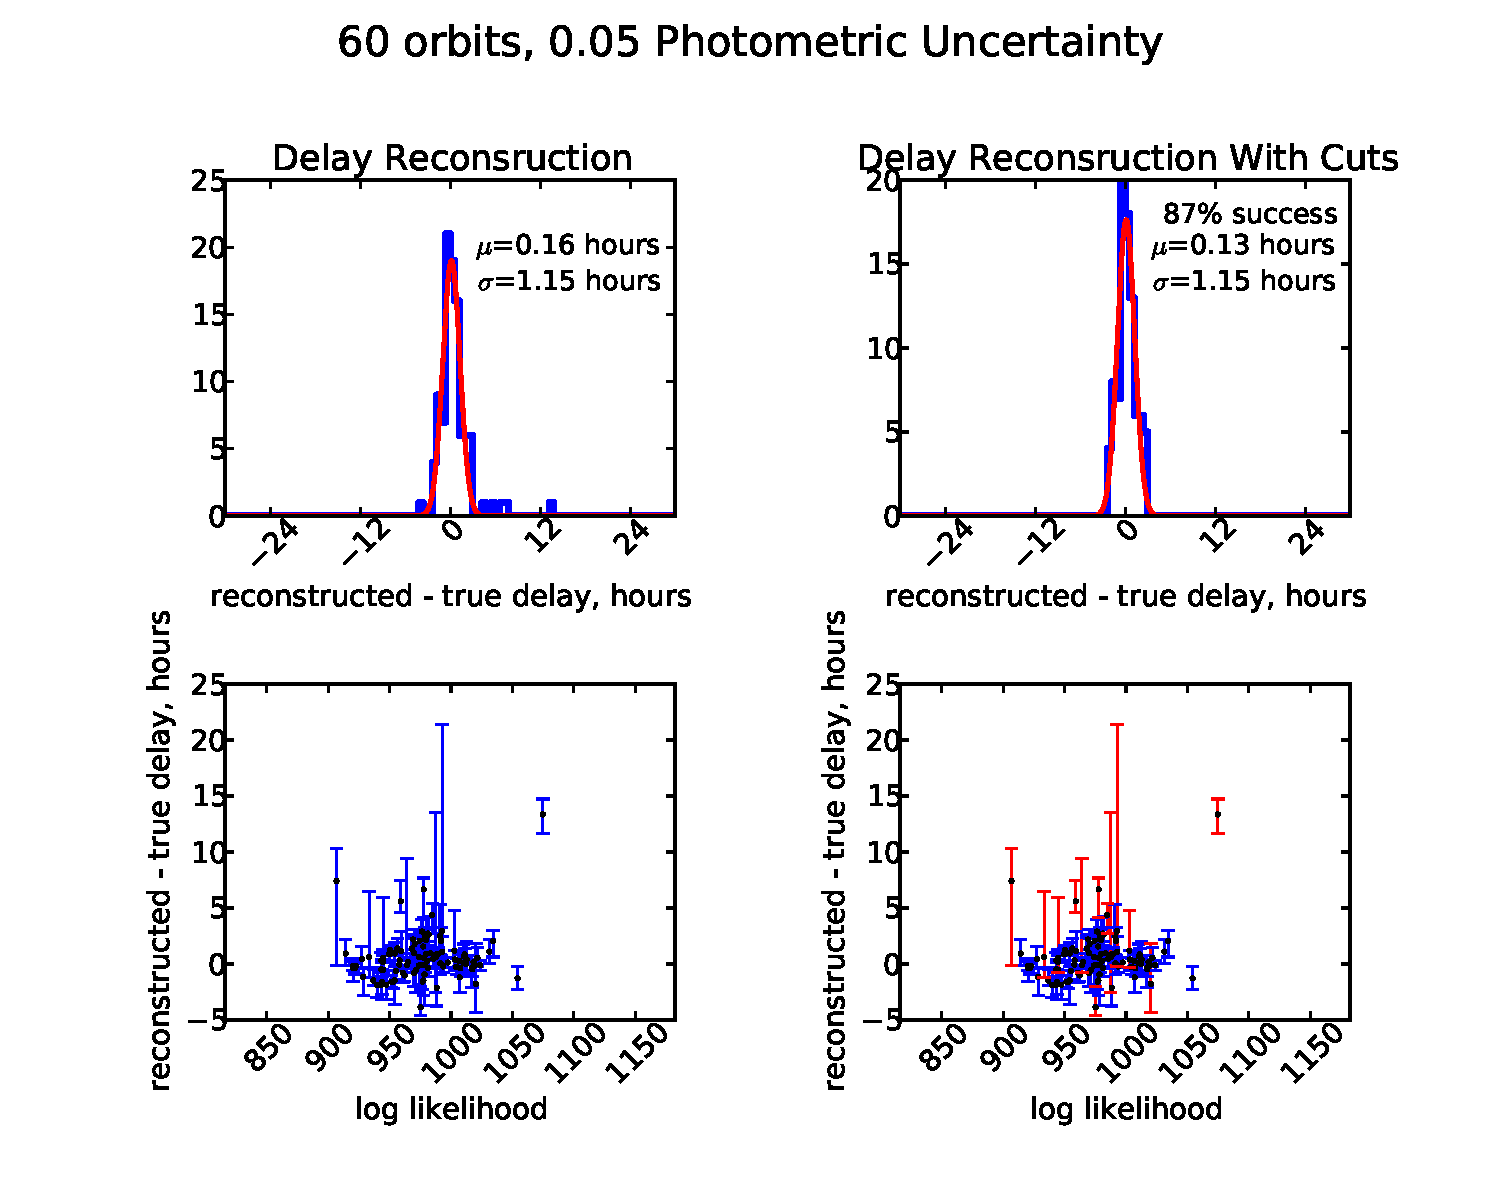
\includegraphics[width=\linewidth]{./ana_ll_example.pdf}
\caption{The systematic behavior of the reconstruction is characterized using the distribution of 100 reconstructed delays. The example shown here is for 60 orbits and a photometric uncertainty of 0.05 mag. The top left shows a distribution of the results with a Gaussian fit with standard deviation $\sigma$. The bottom left shows the delay residuals, with uncertainties derived from the MCMC analysis, vs. the log-likelihood value of the reconstruction. The bottom left figure shows the same plot with the cuts described in the text. The rejected instances are highlighted in red. The top right plot shows the distribution of delay residuals after the rejected instances have been cut out. In this particular example 13\% of the events did not reconstruct with the fidelity required.}\label{fig:volume}
\end{center}
\end{figure}

\begin{figure}[t]
\begin{center}
%\plotone{figures/mastervolume.png}
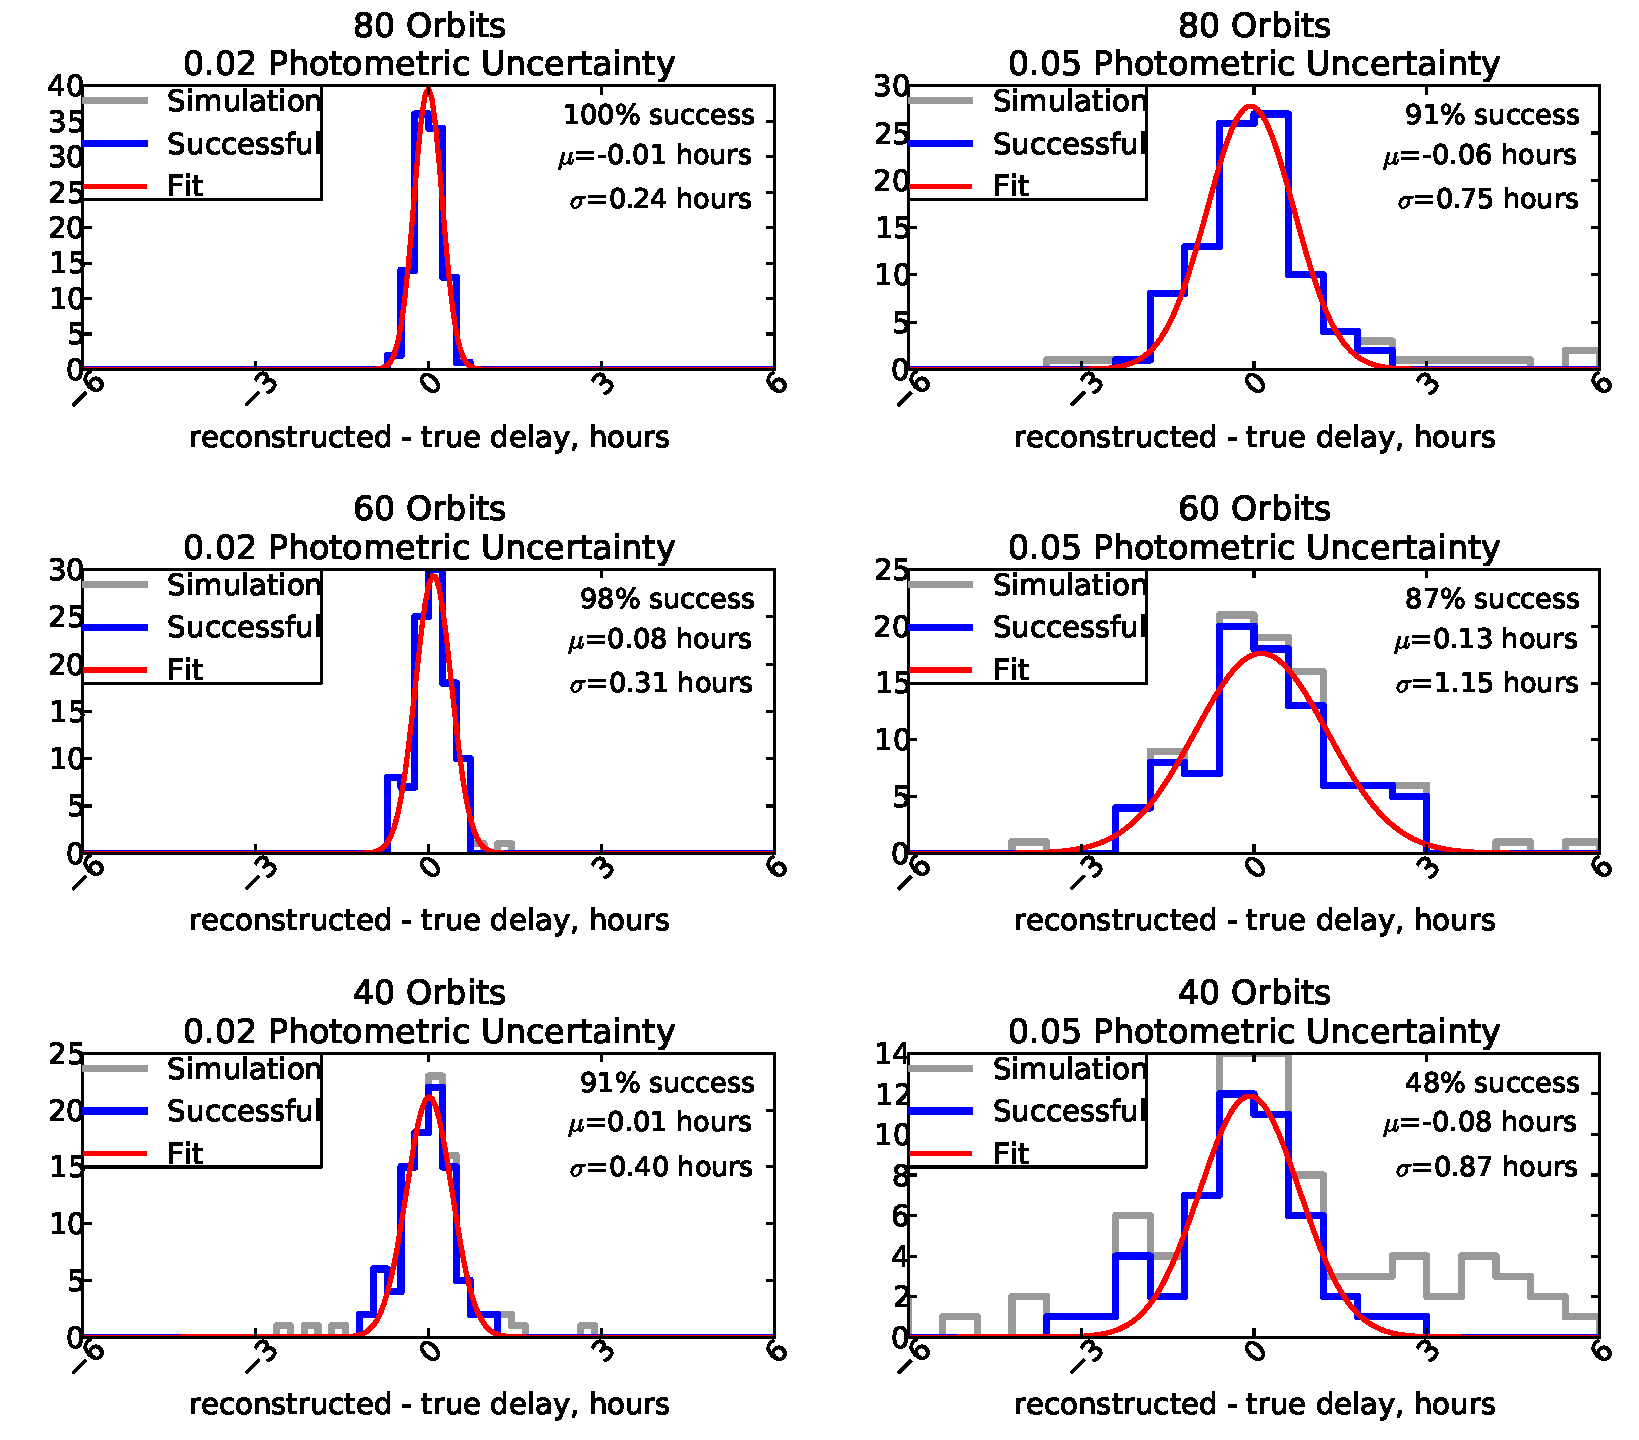
\includegraphics[width=\linewidth]{./systematic_examples.pdf}
\caption{The probability of a successful measurement and resolution are shown for several examples of number of orbits and photomoetric uncertainty. The delay residuals from the simulations are shown in gray. The distribution of successful instances, with the requirements described in the text, are shown in blue. A Gaussian function is fit to the distribution of successful delay reconstructions to obtain the expected delay resolution.}\label{fig:volume}
\end{center}
\end{figure}

\begin{figure}[t]
\begin{center}
%\plotone{figures/mastervolume.png}
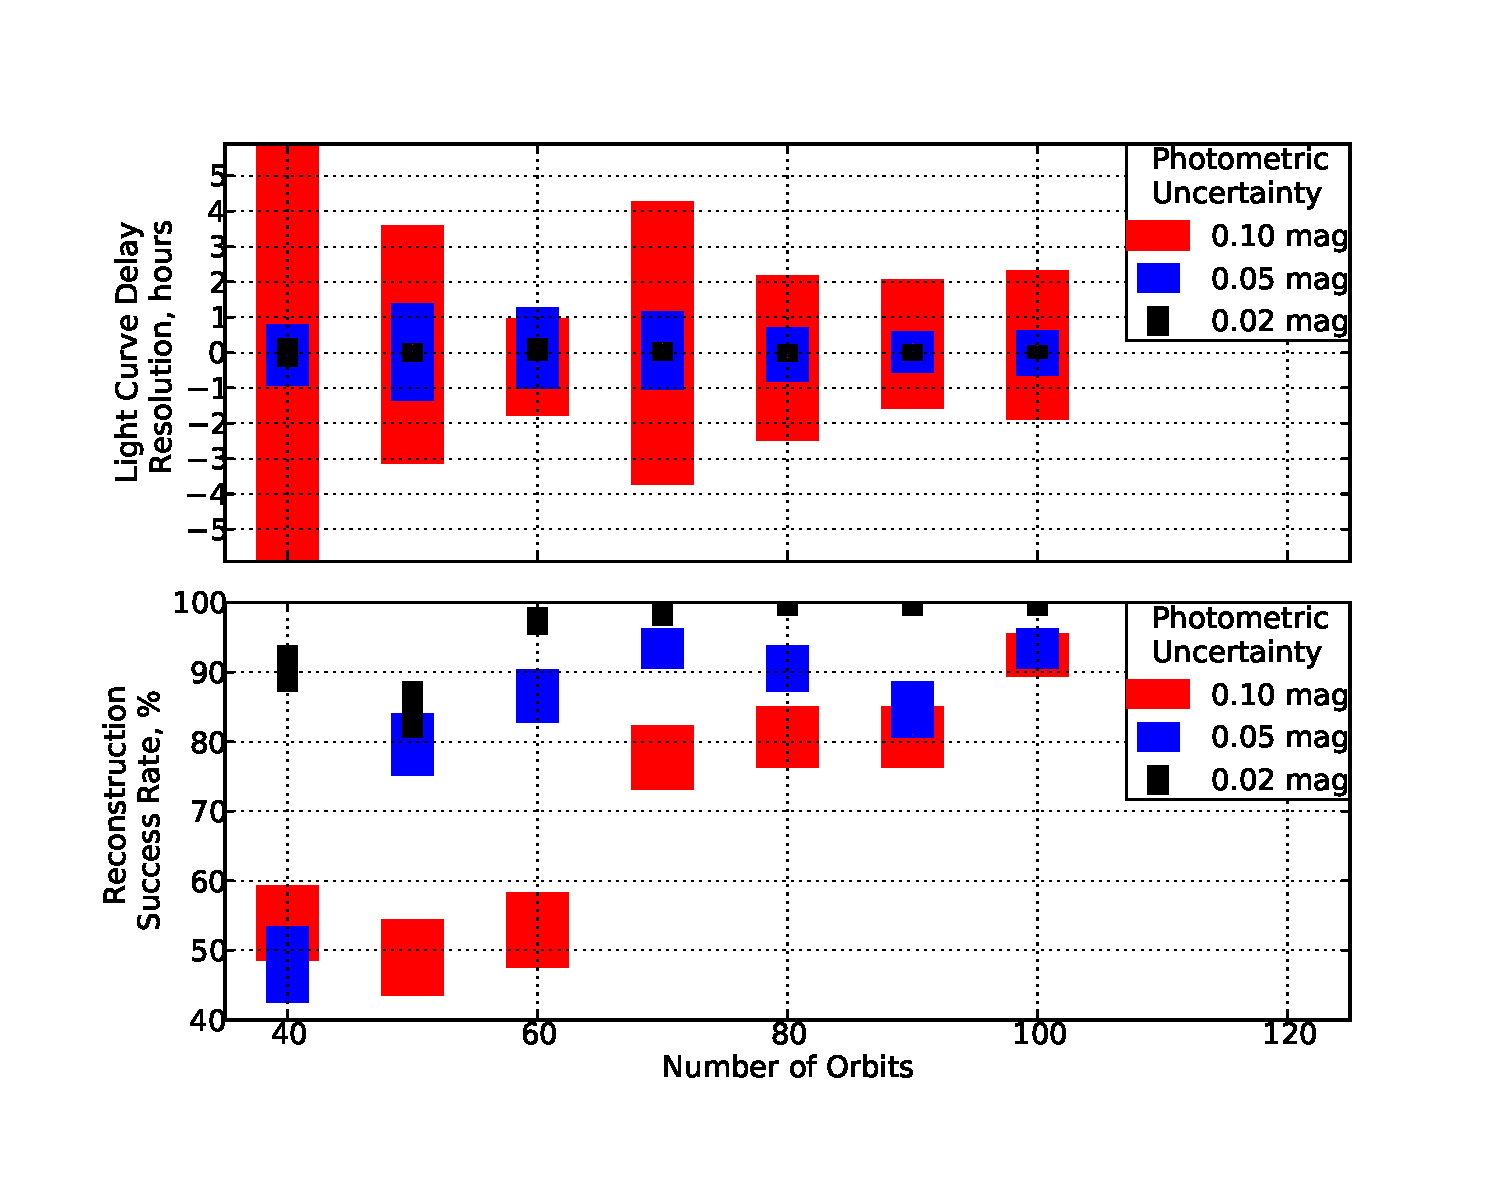
\includegraphics[width=\linewidth]{./systematics_smy.pdf}
\caption{Summary of results for the delay measurement resolution (top panel) reconstruction success rate (bottom panel). Photometric uncertainties of 0.02~mag result in delay resolutions smaller than one day and are down to six hours for 80 orbits and above. Even with photometric uncertainties of 0.05~mag, delay resolutions smaller that 1~day can be achieved. The reconstruction success is 90\% for more than 60 orbits and photometric uncertainties below 0.05~mag.}\label{fig:volume}
\end{center}
\end{figure}

\section{Discussion and Conclusions}\label{sec:disc}

\acknowledgements

This work was carried out at Jet Propulsion Laboratory, California
Institute of Technology, under a contract with NASA.  Thank conversations with Francis-Yan, Chuck Keeton, Frederic Courbin. 

\bibliographystyle{apj}

\bibliography{/Users/leonidas/Dropbox/bibdesk/moustakasbibs}

\end{document}

